\subsubsection{Общая структура програмной компоненты}
\begin{figure}[ht!]
    \centering
    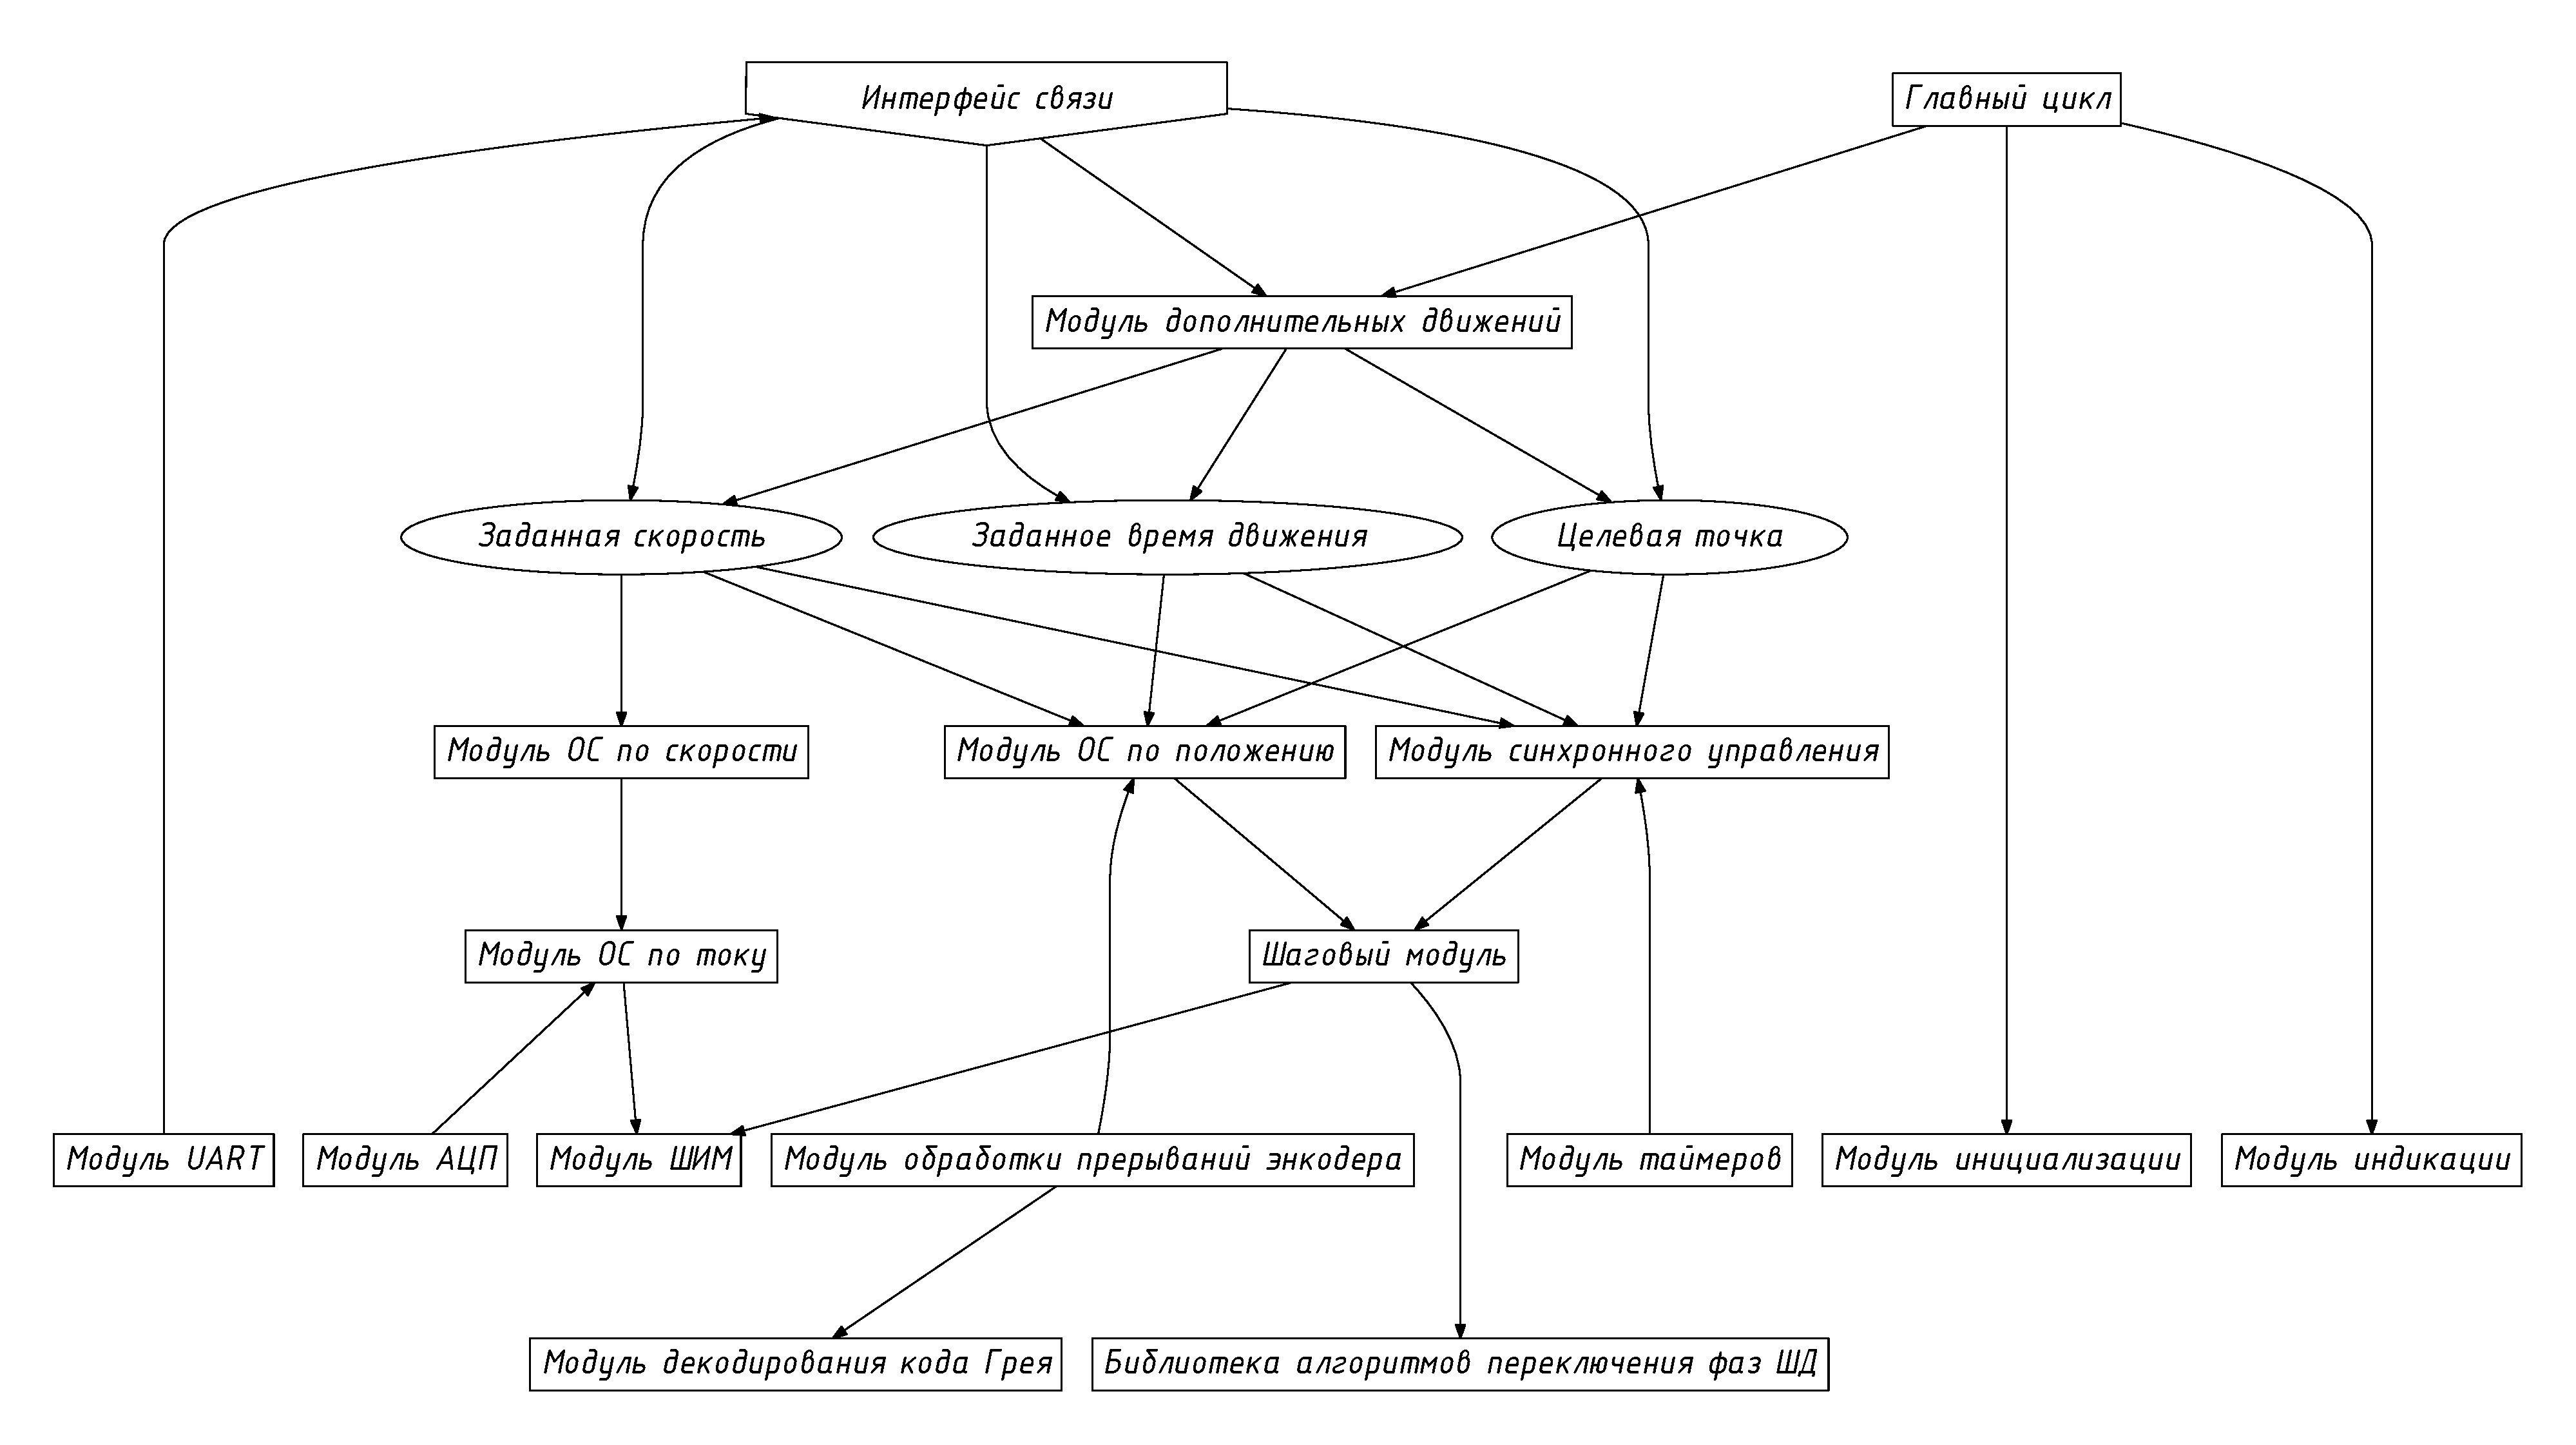
\includegraphics[width=1.3\linewidth,
                     angle=90,
                     trim=0mm 100mm 0mm 100mm]
                    {src/pictures/soft_arch.pdf}
    \caption{Архитектура програмной компоненты}
    \label{pic_soft_arch}
\end{figure}
Любою траекторию, даже достаточно сложную, с остановками и процессами плавного
разгона и торможения можно разбить на простые линейные отрезки, на которых можно
считать постоянными скорость или ускорение. Тем самым, упростим нашу траекторию
до кусочно линейной кривой, линейные отрезки граничат друг с другом через
некоторые точки в пространстве координат время~--~угол~--~скорость.
Движение на каждом участке задаем 2 из 3 координат:

\begin{enumerate}
    \item Время движения~--- точка на временной оси, когда закончится отрезок
    \item Скорость~--- если указано, то система будет поддерживать в движении
        постоянную скорость
    \item Целевая точка~--- точка в пространстве координаты движения, где
        закончится отрезок
\end{enumerate}
Соответственно движение на каждом участке определяется целиком 2мя узлами,
предыдущим~-- начальные условия, и следующим~-- конечные условия.

Структура програмного обеспечения для микроконтролера строилась слоями,
диффиренцироваными по отвественности:

\begin{enumerate}
    \item Задающий~--- фактически в пределах привода инициатор движения. Может
        либо сам задавать параметры текущего отрезка движения, либо выбрать один
        из предопределенных сценариев движения из модуля дополнительных
        движений (см. разд. \ref{module_elementary_motions})

    \item Активный исполнительный алгоритм~--- через единый интерфейс
        сосуществуют два алгоритма смены шагов:
        \begin{enumerate}
            \item Модуль управления по энкодеру (см. разд.
                \ref{module_feedback_control_desc} и разд.
                \ref{module_control_modules_feedback_control})
            \item Модуль синхронного управления (см. разд.
                \ref{module_synchronized_control_desc} и разд.
                \ref{module_control_modules_synchronized_control})
        \end{enumerate}
        Единовременно работает только один алгоритм. Главная разница между ними
        состоит в принципе определения момента переключения обмоток в
        последовательности. Иными словами эти модули только определяют момент
        времени переколючения, и направление следующего шага, вызывая при этом
        функцию из следующего уровня.
    \item Алгоритмы исполнения шагов (шаговый модуль) (см. разд.
        \ref{module_control_algo_desc} и разд.
        \ref{module_control_algo})
    \item Аппаратный уровень~--- уровень работы с аппаратной частью
        микроконтролера, платформа зависимая компонента. (см. разд.
            \ref{module_timers},
            \ref{module_pwm_wrap_module},
            \ref{module_init},
            \ref{module_adc},
            \ref{module_led_control},
            % \ref{module_uart}, его пока нет =]
            \ref{module_sensors_encoder})
\end{enumerate}

\subsubsection{Модуль ОС по положению}
\label{module_feedback_control_desc}
Для контура обратной связи по положению был споектирован модуль:
раздел \ref{module_control_modules_feedback_control},
стр. \pageref{module_control_modules_feedback_control}.

Обозначив направление движения как $\textit{dir} = sign(\dot \theta) = \pm 1$ и
объединив формулы для двух направлений движений, получим из
(\ref{movement_zone_posit_dir_for_delta}) и
(\ref{movement_zone_negat_dir_for_delta}) для зоны движения

\begin{equation}
    \label{movement_zone_for_delta}
    \theta_\textit{ком} - \theta_\textit{шаг}
    < dir \cdot (\phi_\textit{акт} - \theta)
    \leq \theta_\textit{ком}
\end{equation}

и из (\ref{switch_zone_posit_dir_for_delta})
и (\ref{switch_zone_negat_dir_for_delta}) для зоны переключения

\begin{equation}
    \label{switch_zone_for_delta}
    \theta_\textit{ком} - 2\theta_\textit{шаг}
    < dir \cdot (\phi_\textit{акт} - \theta)
    \leq \theta_\textit{ком} - \theta_\textit{шаг}
\end{equation}


\subsubsection{Модуль бездатчикового управления}
\label{module_synchronized_control_desc}
Модуль классического управления шаговым двигателем по тамеру, работает на основе
системного таймера микроконтролера и его прерываниях. Фактической задачей модуля
является определения частоты переключения обмоток, проверка что частота не
превосходит предельную (формула. \ref{step_motor_transfer_function}), и
своевременное переключение обмоток согласно расчитанной частоте.

\subsubsection{Шаговый модуль}
\label{module_control_algo_desc}
Шаговый модуль является интерфейсом переключения фаз шагового двигателя и
обладает только одним доступным другим модулям методом~--- методом включения
следующего (или предыдущего, в зависимости от желаемого направления движения)
алгоритмического шага управления двигателем (см. \ref{sec_step_control_algos}
о циклической природе алгоритмических шагов), фактически управляя только
полярностью напряжения, подаваемого на фазы и коэффициентом для уровня ШИМ
сигнала, так как полушаговый алгоритм предполагает уменьшение уровня тока в
обмотках в момент времени когда включены обе фазы на коэффициент $\sqrt{2}$ по
сравнению с шагами когда включена только одна
(см. разд. \ref{section_half_phase_algo}).

Интерфейс модуля:
\lstinputlisting
    [firstline=20, lastline=24]
    {../firmware/SatStepperBegin/control_algo.h}

Модуль может работать в одном из трёх
алгоритмов переключения обмоток~--- однофазном, двухфазном или полуфазном.

Такая структура позволяет полностью изолировать более высокоуровневые модули от
того, как реализуются шаги двигателя, какой алгоритм переключения фаз
используется и т.д., оставляя при этом другим модулям ответственность о таких
вещах как поддержание требуемых токов и т.п.

\subsubsection{Скоростной модуль}
Модуль контроля по скорости в качестве сигнала обратной связи использует
дифференцированый сигнал с энкодера. Дифференцирование происходит неявно,
так как фактически мы измеряем промежуток времени между приходом импульсов с
энкодера. Этот сигнал зашумлен, и требует фильтрации.
Из отрезков времени не трудно получить скорость, взяв обратную величину и
домножив на радиальную меру одного отсчета энкодера. По величине ошибки скорости
корректируется величина поддерживаемого момента.

\subsubsection{Токовый модуль}
Токовый модуль являет собой процессы поддержания постоянным тока в обмотках
статора на протяжении всего шага, пока фаза включена. В качестве сигнала
обратной связи использует результаты работы АЦП 4~--~х датчиков тока.
Пропорционально ошибке корректирует абсолютное значение уровня ШИМ сигнала в
cоответствующем модуле. В этом же модуле производится корректирование сигнала
уровня ШИМ по измерениям напряжения на шине общего питания.
